\documentclass[10pt,letterpaper]{article}
\usepackage[top=0.85in,left=2.75in,footskip=0.75in]{geometry}

% amsmath and amssymb packages, useful for mathematical formulas and symbols
\usepackage{amsmath,amssymb}

% Use adjustwidth environment to exceed column width (see example table in text)
\usepackage{changepage}

% Use Unicode characters when possible
\usepackage[utf8x]{inputenc}

% textcomp package and marvosym package for additional characters
\usepackage{textcomp,marvosym}

% cite package, to clean up citations in the main text. Do not remove.
\usepackage{cite}

% Use nameref to cite supporting information files (see Supporting Information section for more info)
\usepackage{nameref,hyperref}
\usepackage[capitalize]{cleveref}
\usepackage[inline]{enumitem}
\usepackage[per-mode=symbol,group-separator={,},group-minimum-digits=4]{siunitx}
\usepackage{listings}
\usepackage{todonotes}
\usepackage{subcaption}
\usepackage{url}

% line numbers
\usepackage[right]{lineno}

% ligatures disabled
\usepackage{microtype}
\DisableLigatures[f]{encoding = *, family = * }

% color can be used to apply background shading to table cells only
\usepackage{xcolor}

\usepackage[commentmarkup=footnote]{changes}

% array package and thick rules for tables
\usepackage{array}

\usepackage{physics}  % for \norm
\usepackage{graphicx}
\graphicspath{ {../paper_figures} }

% create "+" rule type for thick vertical lines
\newcolumntype{+}{!{\vrule width 2pt}}

% create \thickcline for thick horizontal lines of variable length
\newlength\savedwidth
\newcommand\thickcline[1]{%
  \noalign{\global\savedwidth\arrayrulewidth\global\arrayrulewidth 2pt}%
  \cline{#1}%
  \noalign{\vskip\arrayrulewidth}%
  \noalign{\global\arrayrulewidth\savedwidth}%
}

% \thickhline command for thick horizontal lines that span the table
\newcommand\thickhline{\noalign{\global\savedwidth\arrayrulewidth\global\arrayrulewidth 2pt}%
\hline
\noalign{\global\arrayrulewidth\savedwidth}}

% Remove comment for double spacing
%\usepackage{setspace} 
%\doublespacing

% Text layout
\raggedright
\setlength{\parindent}{0.5cm}
\textwidth 5.25in 
\textheight 8.75in

% Bold the 'Figure #' in the caption and separate it from the title/caption with a period
% Captions will be left justified
\usepackage[aboveskip=1pt,labelfont=bf,labelsep=period,justification=raggedright,singlelinecheck=off]{caption}
\renewcommand{\figurename}{Fig}

% Use the PLoS provided BiBTeX style
\bibliographystyle{plos2015}

% Remove brackets from numbering in List of References
\makeatletter
\renewcommand{\@biblabel}[1]{\quad#1.}
\makeatother


% Header and Footer with logo
\usepackage{lastpage,fancyhdr,graphicx}
\usepackage{epstopdf}
%\pagestyle{myheadings}
\pagestyle{fancy}
\fancyhf{}
%\setlength{\headheight}{27.023pt}
%\lhead{\includegraphics[width=2.0in]{PLOS-submission.eps}}
\rfoot{\thepage/\pageref{LastPage}}
\renewcommand{\headrulewidth}{0pt}
\renewcommand{\footrule}{\hrule height 2pt \vspace{2mm}}
\fancyheadoffset[L]{2.25in}
\fancyfootoffset[L]{2.25in}
\lfoot{\today}

\begin{document}
\vspace*{0.2in}

% Title must be 250 characters or less.
\begin{flushleft}
{\Large
\textbf\newline{Supplemental Material: Multidimensional analysis and detection of informative features in human brain white matter} % Please use "sentence case" for title and headings (capitalize only the first word in a title (or heading), the first word in a subtitle (or subheading), and any proper nouns).
}
\newline
% Insert author names, affiliations and corresponding author email (do not include titles, positions, or degrees).
\\
Adam Richie-Halford\textsuperscript{1*},
Jason Yeatman\textsuperscript{2},
Noah Simon\textsuperscript{3},
Ariel Rokem\textsuperscript{4},
\\
\bigskip
\textbf{1} eScience Institute, University of Washington, Seattle, WA, USA
\\
\textbf{2} Graduate School of Education and Division of Developmental and Behavioral Pediatrics, Stanford University, Stanford, CA, USA
\\
\textbf{3} Department of Biostatistics, University of Washington, Seattle, WA, USA
\\
\textbf{4} Department of Psychology, University of Washington, Seattle, WA, USA
\\
\bigskip

% Insert additional author notes using the symbols described below. Insert symbol callouts after author names as necessary.
% Use the asterisk to denote corresponding authorship and provide email address in note below.
* richford@uw.edu

\end{flushleft}

\section{Bundle and coefficient profiles}
\label{sec:bundle-profiles}

Here, we present the bundle profiles and $\hat{\beta}$ coefficients
for each dataset. Throughout this section, diffusion metrics are plotted
along the length of eighteen bundles:
right corticospinal (CSTR),
left corticospinal (CSTL),
right uncinate (UNCR),
left uncinate (UNCL),
left inferior fronto-occipital fasciculus (IFOL),
right inferior fronto-occipital fasciculus (IFOR),
right arcuate (ARCR),
left arcuate (ARCL),
right thalamic radiation (ATRR),
left thalamic radiation (ATRL),
right cingulum cingulate (CGCR),
left cingulum cingulate (CGCL),
callosum forceps posterior (CFP),
callosum forceps anterior (CFA),
right inferior longitudinal fasciculus (ILFR),
left inferior longitudinal fasciculus (ILFL),
right superior longitudinal fasciculus (SLFR),
and left superior longitudinal fasciculus (SLFL).
We display results for two different diffusion metrics: fractional anisotropy
(FA) and mean diffusivity (MD), which are extracted from different diffusion
models depending on the dataset: diffusion tensor imaging (DTI) for the ALS
and WH datasets and diffusion kurtosis imaging (DKI) for the HBN and Cam-CAN
datasets \cite{jensen2005diffusion}. The diffusion metric is always plotted
on the left $y$-axis while the $\hat{\beta}$ coefficients are displayed on
the twin axis on the right-hand-side. The scale of the $\hat{\beta}$-axis is
shared between the FA and MD metrics so that one can compare the relative
imporance of each metric.

\subsection{ALS bundle profiles}

\Cref{fig:als-bp:fa,fig:als-bp:md} show the bundle profiles and regression
coefficients for the ALS dataset FA and MD metrics, respectively. These
figures reinforce the findings in the main text that ALS is localized to the
corticospinal tract. In this study, SGL selected the right corticospinal
tract (CSTR) as important and regularized coefficients in the CSTL. Yet,
\cref{fig:als-bp:fa} also shows group FA differences in the CSTL. This
highlighted a potential drawback of the SGL method, discussed in the main
text in the context of age regression. Namely, SGL is not guaranteed to
identify \emph{all} important features. In this case, if the diagnostic
signal in the CSTL is redundant to that in the CSTR, SGL will regularize the
CSTL features, thereby reducing its sparsity penalty without any
corresponding increase in loss. This parsimony cuts both ways; it is a
feature of the method when one seeks an efficient predictive model, but is a
disadvantage of the method when one wants an exhaustive explanation of feature
importance. We will use the phrase ``parsimony pitfall'' to refer to the
case when SGL regularizes away redundant but obviously important features.

\begin{figure}
    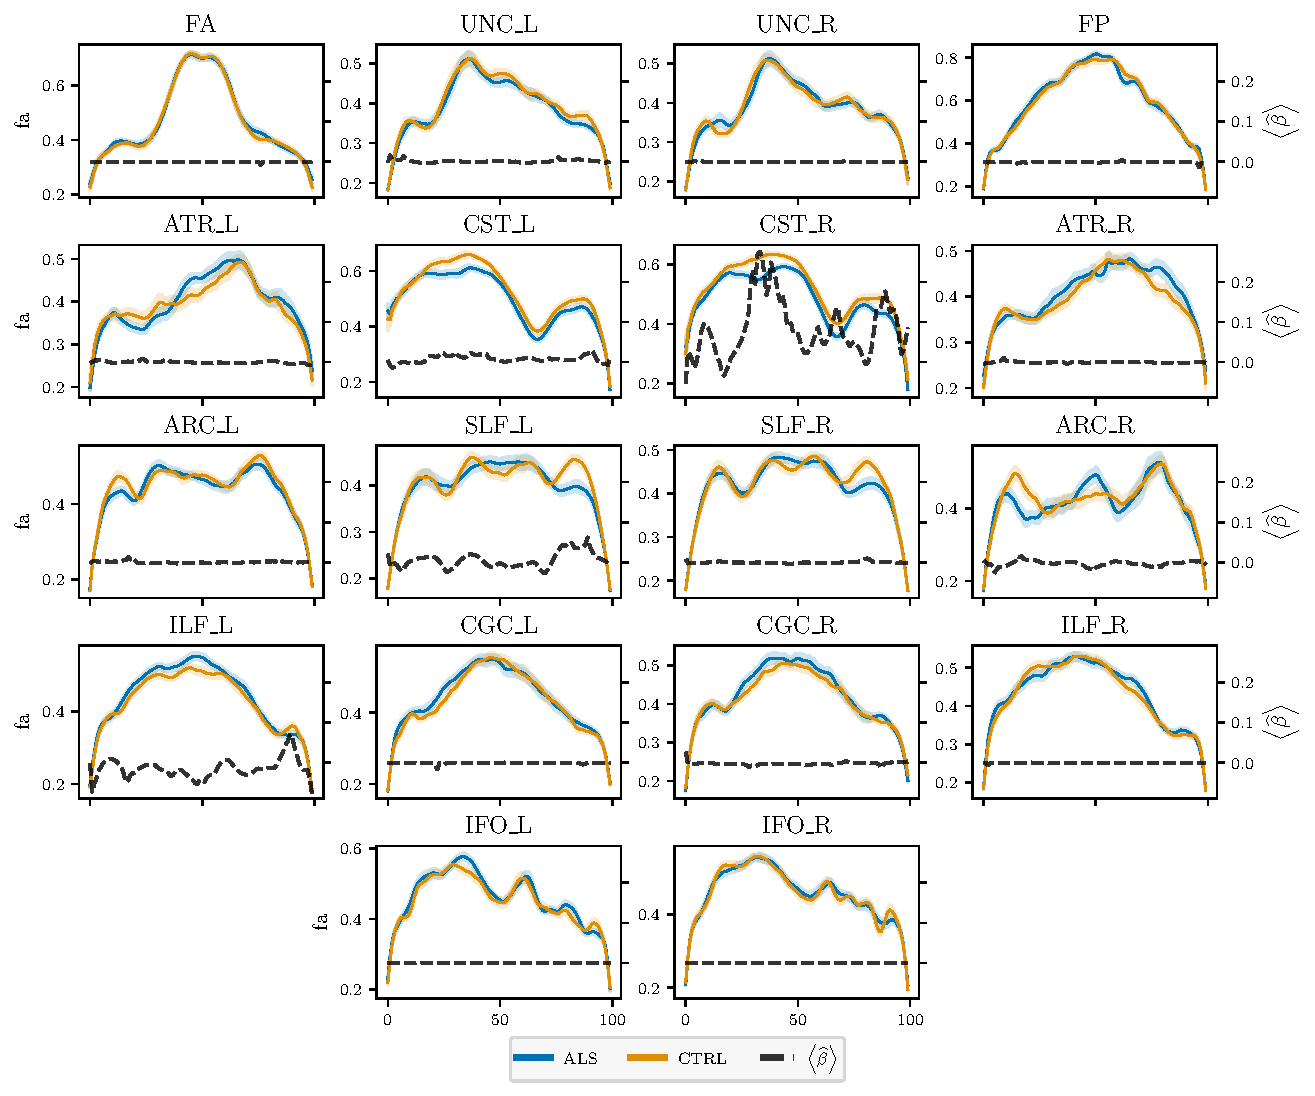
\includegraphics[width=0.9\textwidth]{sarica_coefs_profiles_fa.pdf}
    \caption{%
        {%
            \bf Fractional anisotropy (FA) bundle profiles and $\hat{\beta}$
            coefficients for ALS classification.
        }
        \label{fig:als-bp:fa}
    }
\end{figure}

\begin{figure}
    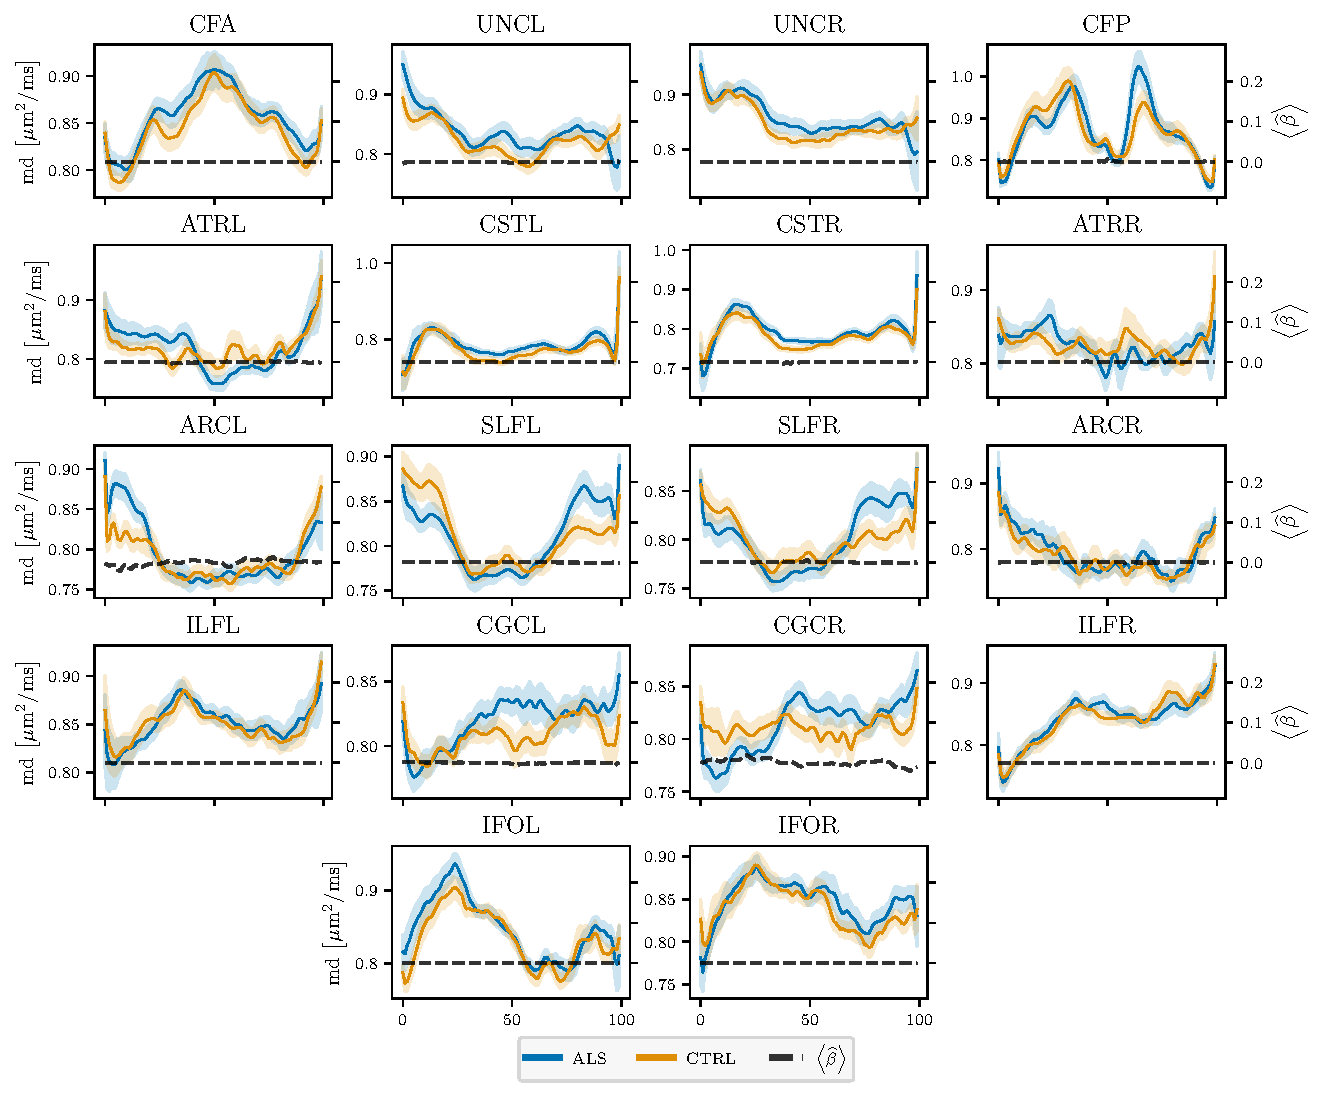
\includegraphics[width=0.9\textwidth]{sarica_coefs_profiles_md.pdf}
    \caption{%
        {%
            \bf Mean diffusivity (MD) Bundle profiles and $\hat{\beta}$
            coefficients for ALS classification.
        }
        \label{fig:als-bp:md}
    }
\end{figure}

\subsection{WH bundle profiles}

\Cref{fig:wh-bp:fa,fig:wh-bp:md} show the bundle profiles and regression
coefficients for the WH dataset. In contrast to the ALS classification case,
the $\hat{\beta}$ coefficients are distributed widely through the brain, supporting
the interpretation that aging is a large and continuous whole-brain process.
These figures also show that SGL behaves much more like the lasso than the group
lasso, as discussed in the main text. The parsimony pitfall is most evident in
the IFOL and IFOR bundles in \cref{fig:wh-bp:md}.

\begin{figure}
    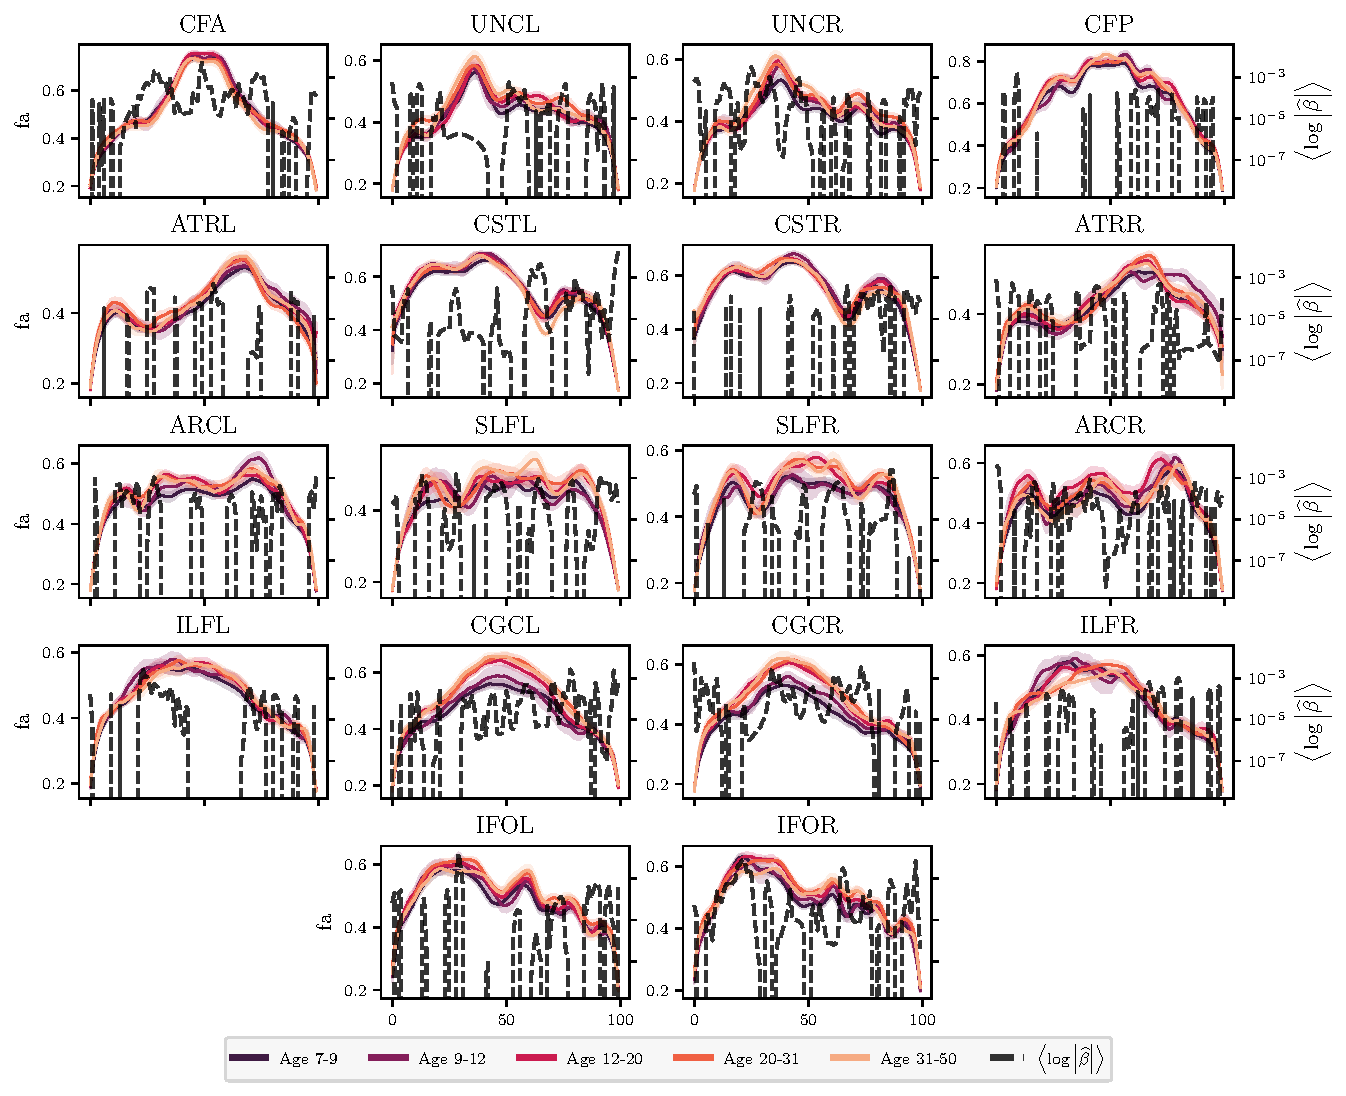
\includegraphics[width=0.9\textwidth]{wh_coefs_profiles_fa.pdf}
    \caption{%
        {%
            \bf Fractional anisotropy (FA) bundle profiles and $\hat{\beta}$
            coefficients for age regression in the WH dataset.
        }
        \label{fig:wh-bp:fa}
    }
\end{figure}

\begin{figure}
    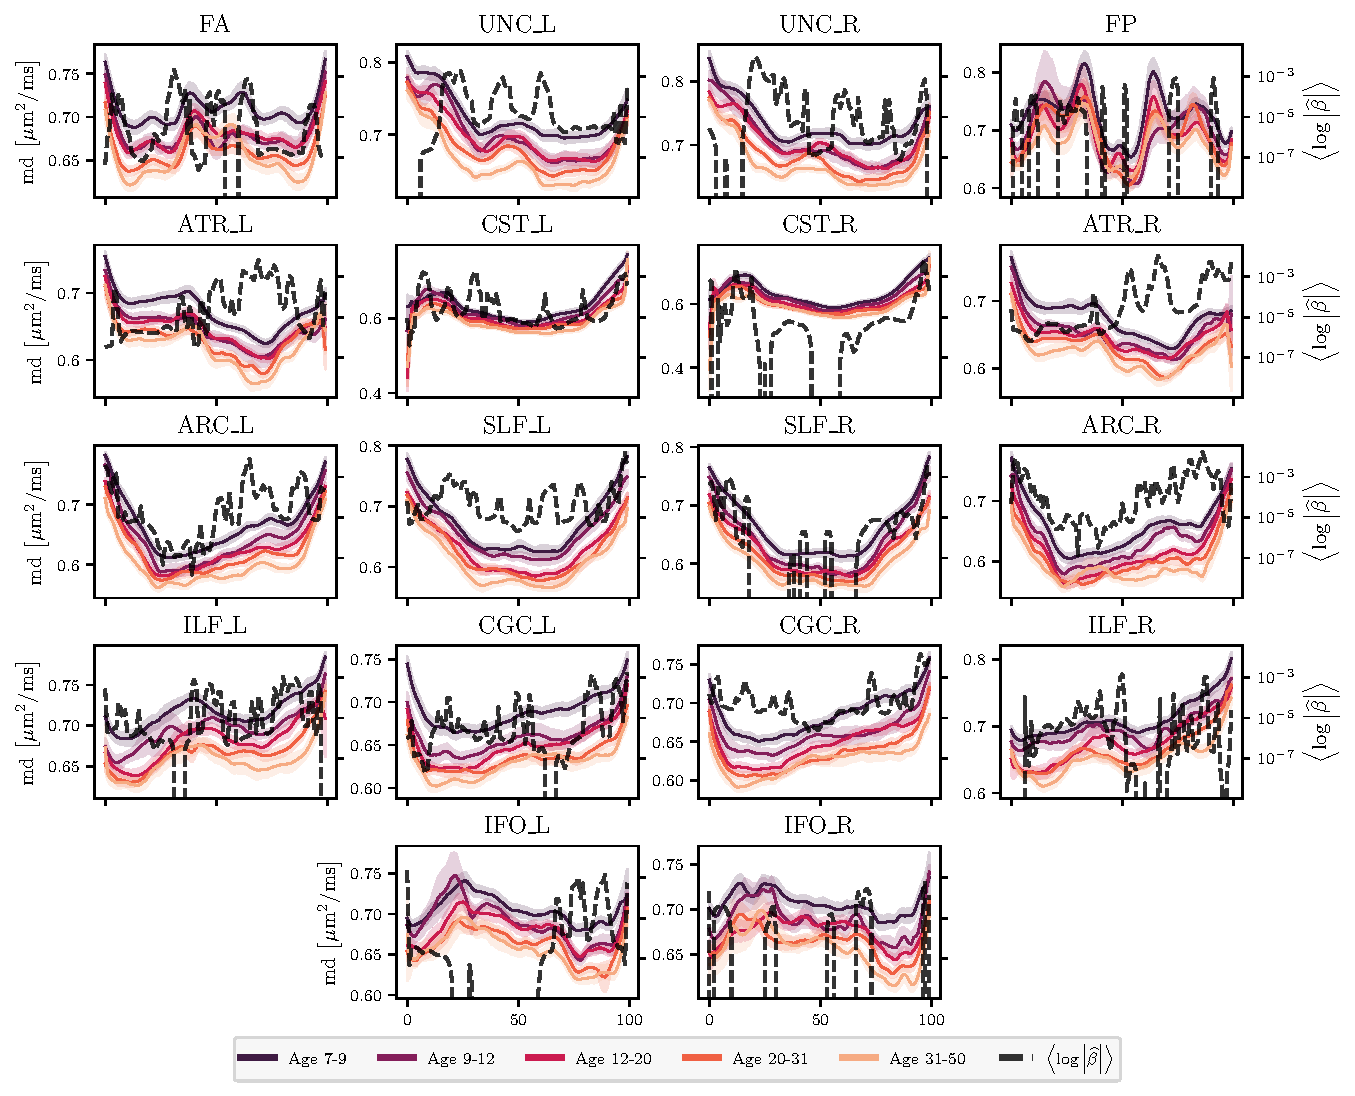
\includegraphics[width=0.9\textwidth]{wh_coefs_profiles_md.pdf}
    \caption{%
        {%
            \bf Mean diffusivity (MD) bundle profiles and $\hat{\beta}$
            coefficients for age regression in the WH dataset.
        }
        \label{fig:wh-bp:md}
    }
\end{figure}

\subsection{HBN bundle profiles}

\Cref{fig:hbn-bp:fa,fig:hbn-bp:md} show the bundle profiles and regression
coefficients for the HBN dataset. Like the WH dataset, the $\hat{\beta}$
coefficients are distributed widely through the brain and SGL behaves more
like the lasso than the group lasso. In contrast the the WH results,
the bundle profiles show different behaviors. For example the SLFL and SLFR
bundle profiles in \cref{fig:wh-bp:md} and \cref{fig:hbn-bp:md} have
different concavity. This is unsurprising, however, given the differences
between these datasets
\begin{enumerate*}[%
    label=(\roman*),%
    before=\unskip{: },%
    itemjoin={{, }},%
    itemjoin*={{, and }}]
    \item different diffusion models, with DTI for the WH dataset and DKI for
    the HBN and Cam-CAN datasets
    \item different age ranges and distributions (which is evident in the
    figure legends), with HBN being a developmental dataset, while WH and Cam-CAN are
    lifespan maturation datasets
    \item different anatomical extents, with the WH streamlines truncated to
    remain with the bundle's bounding regions of interest (the default
    behavior in the legacy \texttt{mAFQ}) and the HBN and Cam-CAN streamlines
    allowed to retain their full extent from whole-brain tractography (the
    default behavior in \texttt{pyAFQ}).
\end{enumerate*}
Thus, one should use caution when comparing bundle profiles and $\hat{\beta}$
coefficients between the WH, HBN, and Cam-CAN models.
The parsimony pitfall is most evident in the UNCL, UNCR, ARCL, SLFL, and
SLFR bundles in \cref{fig:hbn-bp:md}.

\begin{figure}
    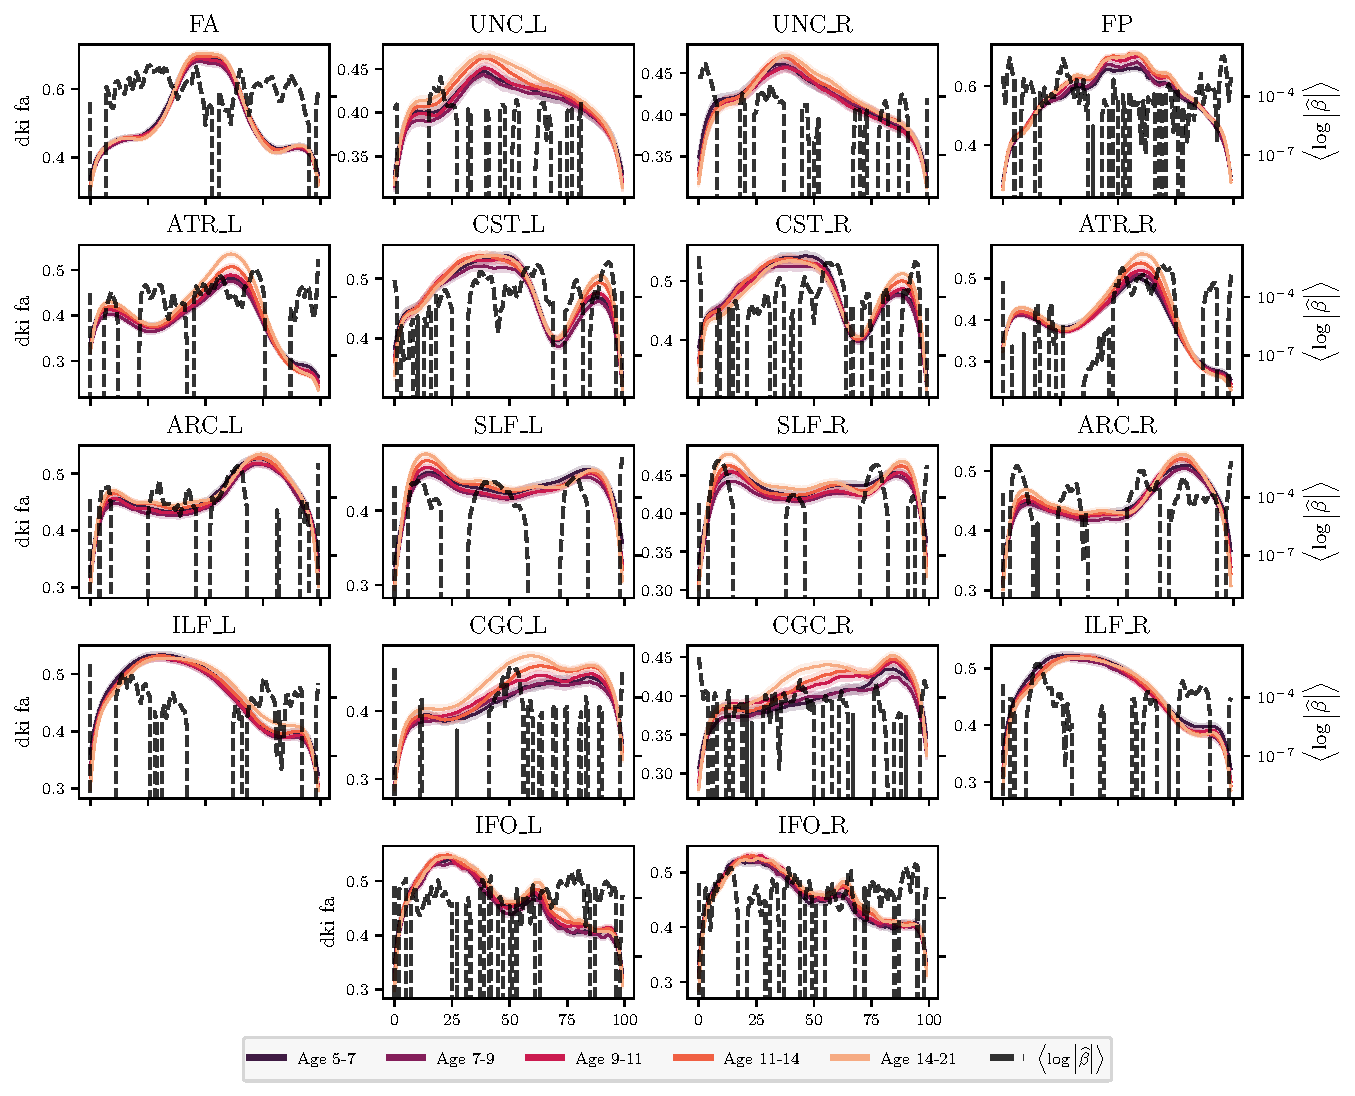
\includegraphics[width=0.9\textwidth]{hbn_coefs_profiles_fa.pdf}
    \caption{%
        {%
            \bf Fractional anisotropy (FA) bundle profiles and $\hat{\beta}$
            coefficients for age regression in the HBN dataset.
        }
        \label{fig:hbn-bp:fa}
    }
\end{figure}

\begin{figure}
    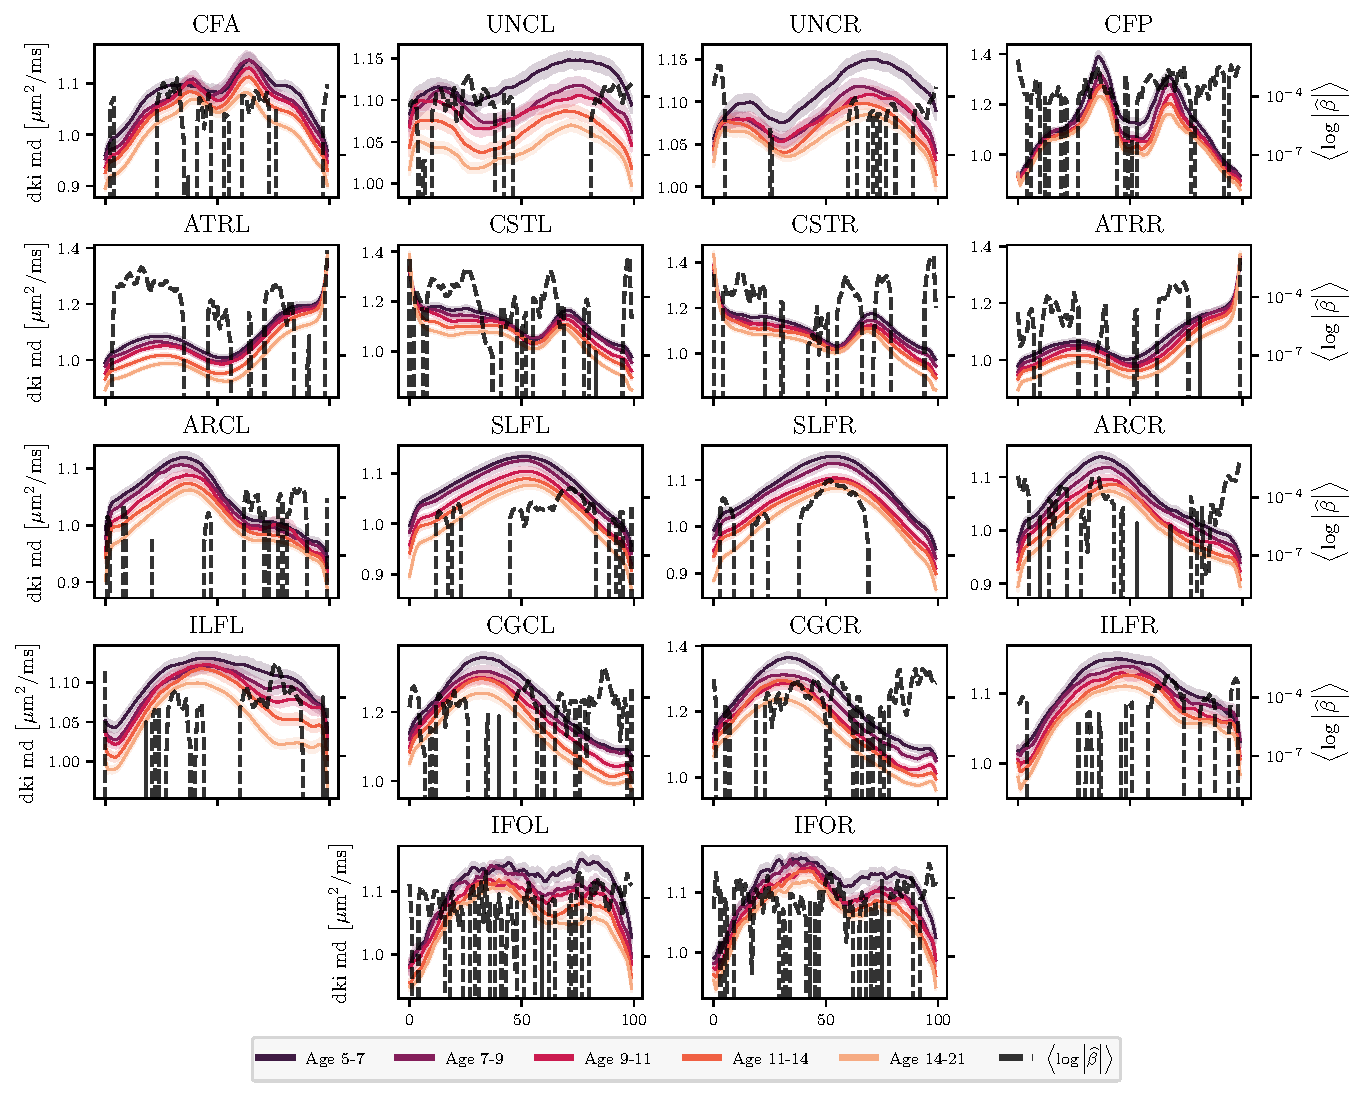
\includegraphics[width=0.9\textwidth]{hbn_coefs_profiles_md.pdf}
    \caption{%
        {%
            \bf Mean diffusivity (MD) bundle profiles and $\hat{\beta}$
            coefficients for age regression in the HBN dataset.
        }
        \label{fig:hbn-bp:md}
    }
\end{figure}

\subsection{Cam-CAN bundle profiles}

\Cref{fig:cc-bp:fa,fig:cc-bp:md} show the bundle profiles and regression
coefficients for the Cam-CAN dataset. Like the WH and HBN datasets, the
$\hat{\beta}$ coefficients are distributed widely through the brain and SGL
behaves more like the lasso than the group lasso. As before, one must be
cautious about comparing bundle profiles and $\hat{\beta}$ coefficients
between models. While the HBN and Cam-CAN datasets share the same diffusion
model and refrain from clipping streamlines, the age distributions for the
two are roughly disjoint, with the WH age distribution straddling the two.
The parsimony pitfall is again evident in the UNCL, UNCR, ARCL, SLFL, and
SLFR bundles in \cref{fig:cc-bp:md}.

\begin{figure}
    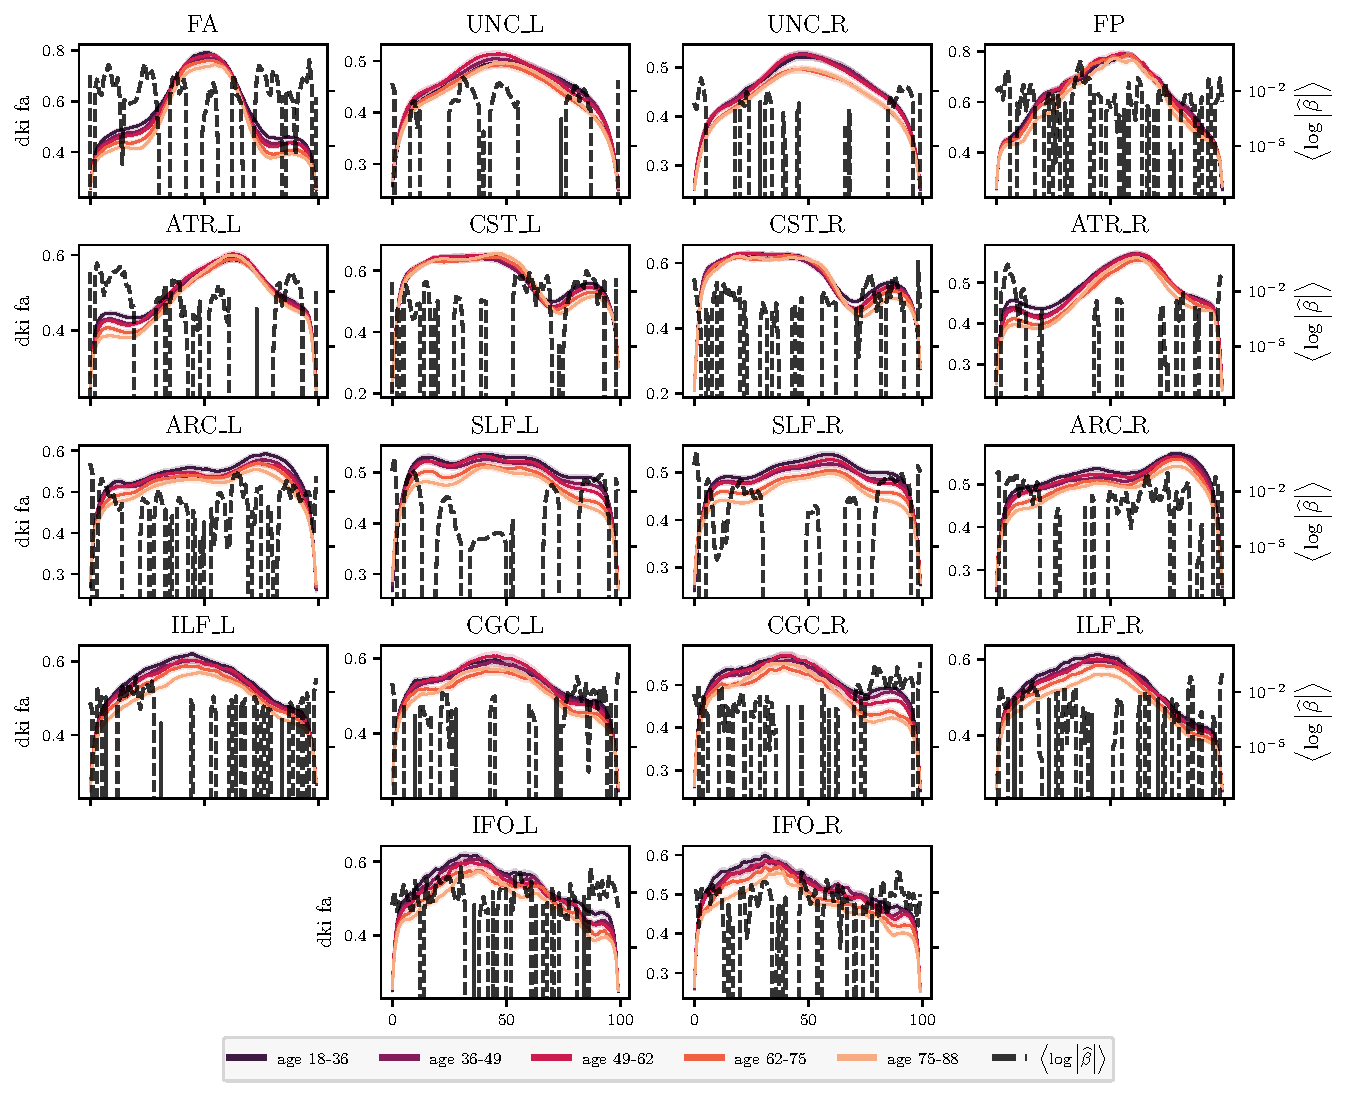
\includegraphics[width=0.9\textwidth]{cc_coefs_profiles_fa.pdf}
    \caption{%
        {%
            \bf Fractional anisotropy (FA) bundle profiles and $\hat{\beta}$
            coefficients for age regression in the Cam-CAN dataset.
        }
        \label{fig:cc-bp:fa}
    }
\end{figure}

\begin{figure}
    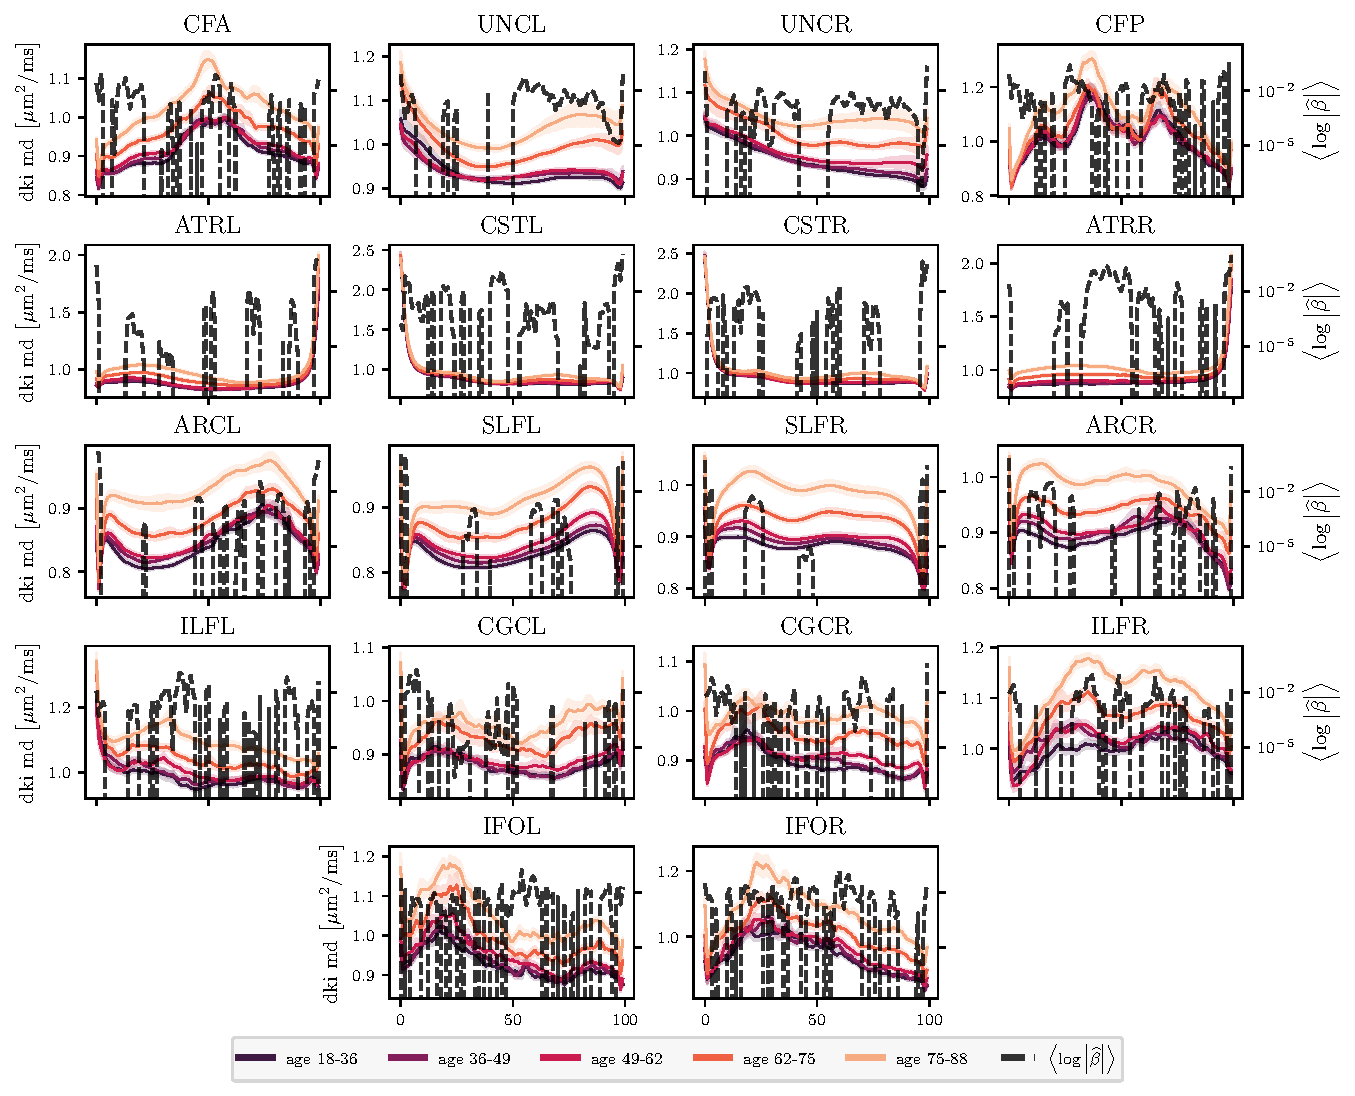
\includegraphics[width=0.9\textwidth]{cc_coefs_profiles_md.pdf}
    \caption{%
        {%
            \bf Mean diffusivity (MD) bundle profiles and $\hat{\beta}$
            coefficients for age regression in the Cam-CAN dataset.
        }
        \label{fig:cc-bp:md}
    }
\end{figure}

\section{Data harmonization in the HBN dataset}

\Cref{fig:hbn-site-bp:fa,fig:hbn-site-bp:md} show the bundle profiles for the HBN dataset separated by scanner site: Rutgers Rutgers University Brain Imaging Center (RU) and the CitiGroup Cornell Brain Imaging Center (CBIC). We see strong site differences in both FA and MD profiles. Conversely, \cref{fig:hbn-site-age-dist} shows that the age distributions at each site are similar. ComBat effectively harmonizes the scanner site differences, as shown in \cref{fig:hbn-harmonized-bp:fa,fig:hbn-harmonized-bp:md}.

\begin{figure}
    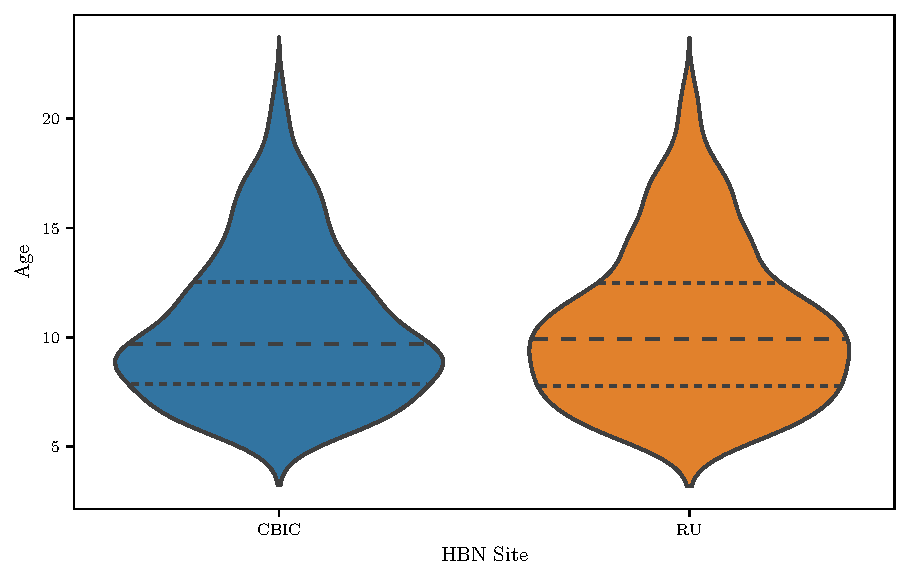
\includegraphics[width=0.9\textwidth]{hbn_site_age_distributions.pdf}
    \caption{%
        {%
            \bf Age distributions are similar between the different
            HBN sites.
        }
        \label{fig:hbn-site-age-dist}
    }
\end{figure}

\begin{figure}
    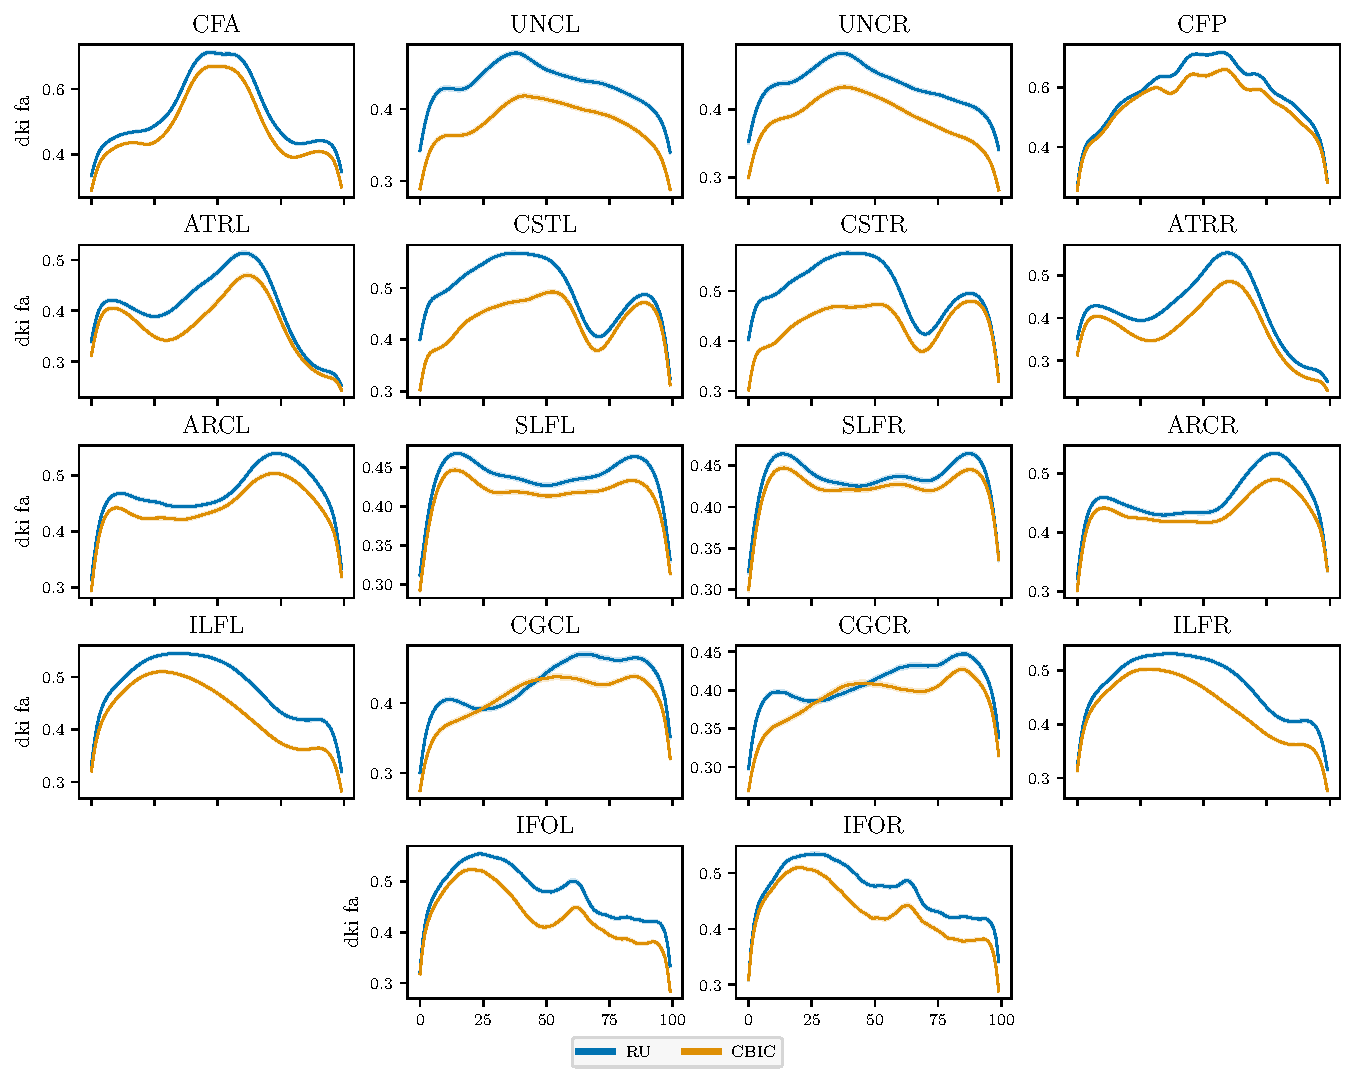
\includegraphics[width=0.9\textwidth]{hbn_site_profiles_fa.pdf}
    \caption{%
        {%
            \bf Fractional anisotropy (FA) bundle profiles
            exhibit strong site differences in the HBN dataset.
        }
        \label{fig:hbn-site-bp:fa}
    }
\end{figure}

\begin{figure}
    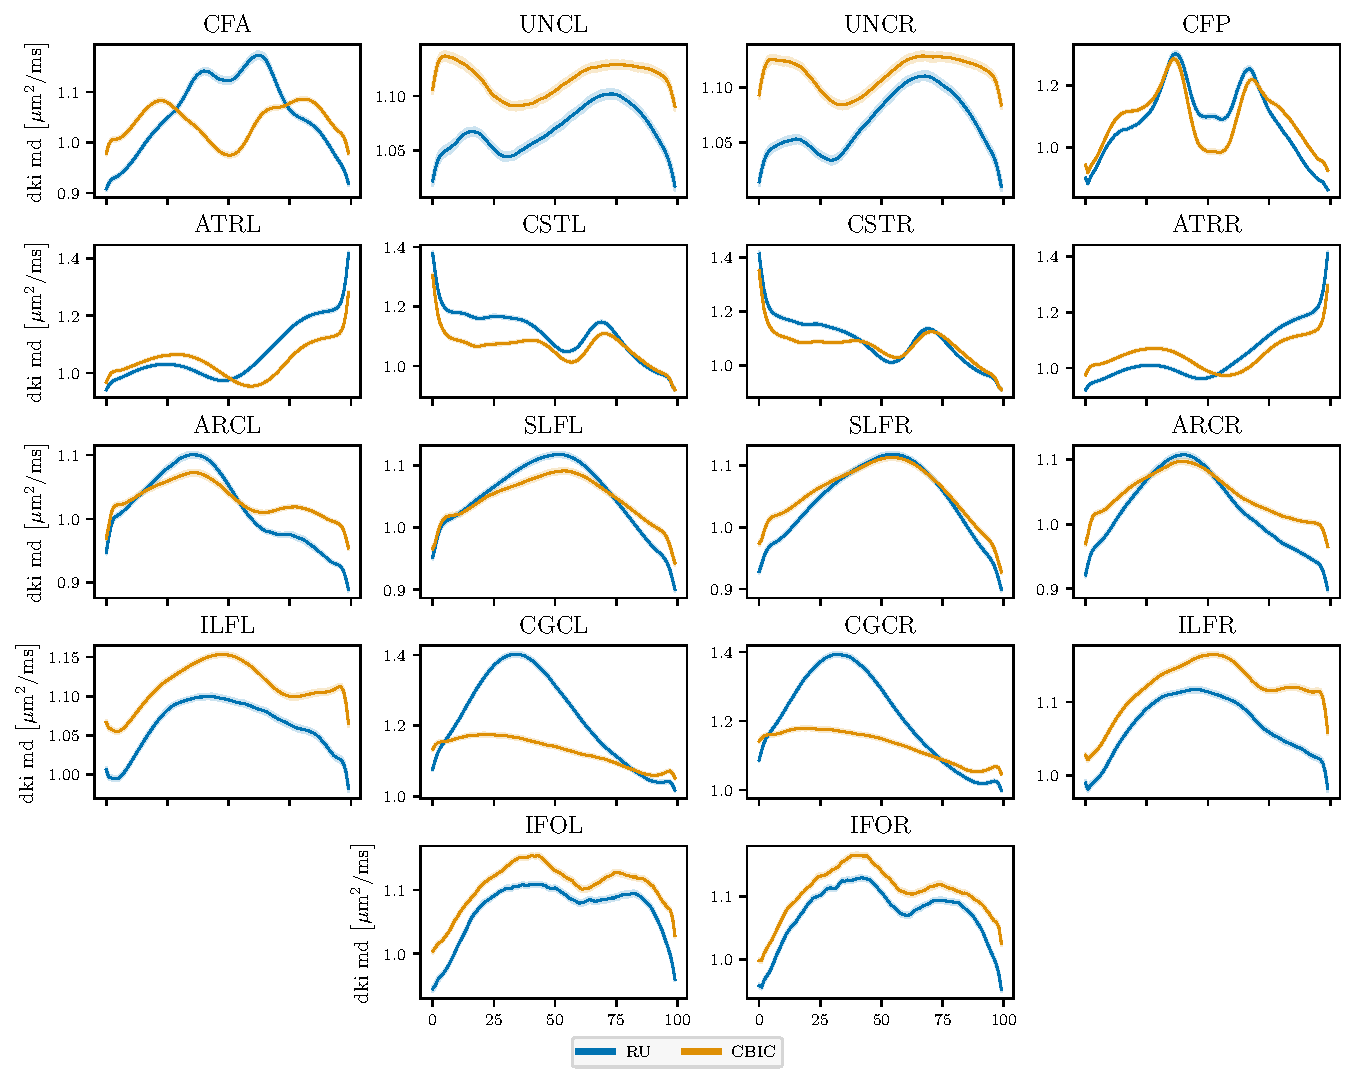
\includegraphics[width=0.9\textwidth]{hbn_site_profiles_md.pdf}
    \caption{%
        {%
            \bf Mean diffusivity (MD) bundle profiles
            exhibit strong site differences in the HBN dataset.
        }
        \label{fig:hbn-site-bp:md}
    }
\end{figure}

\begin{figure}
    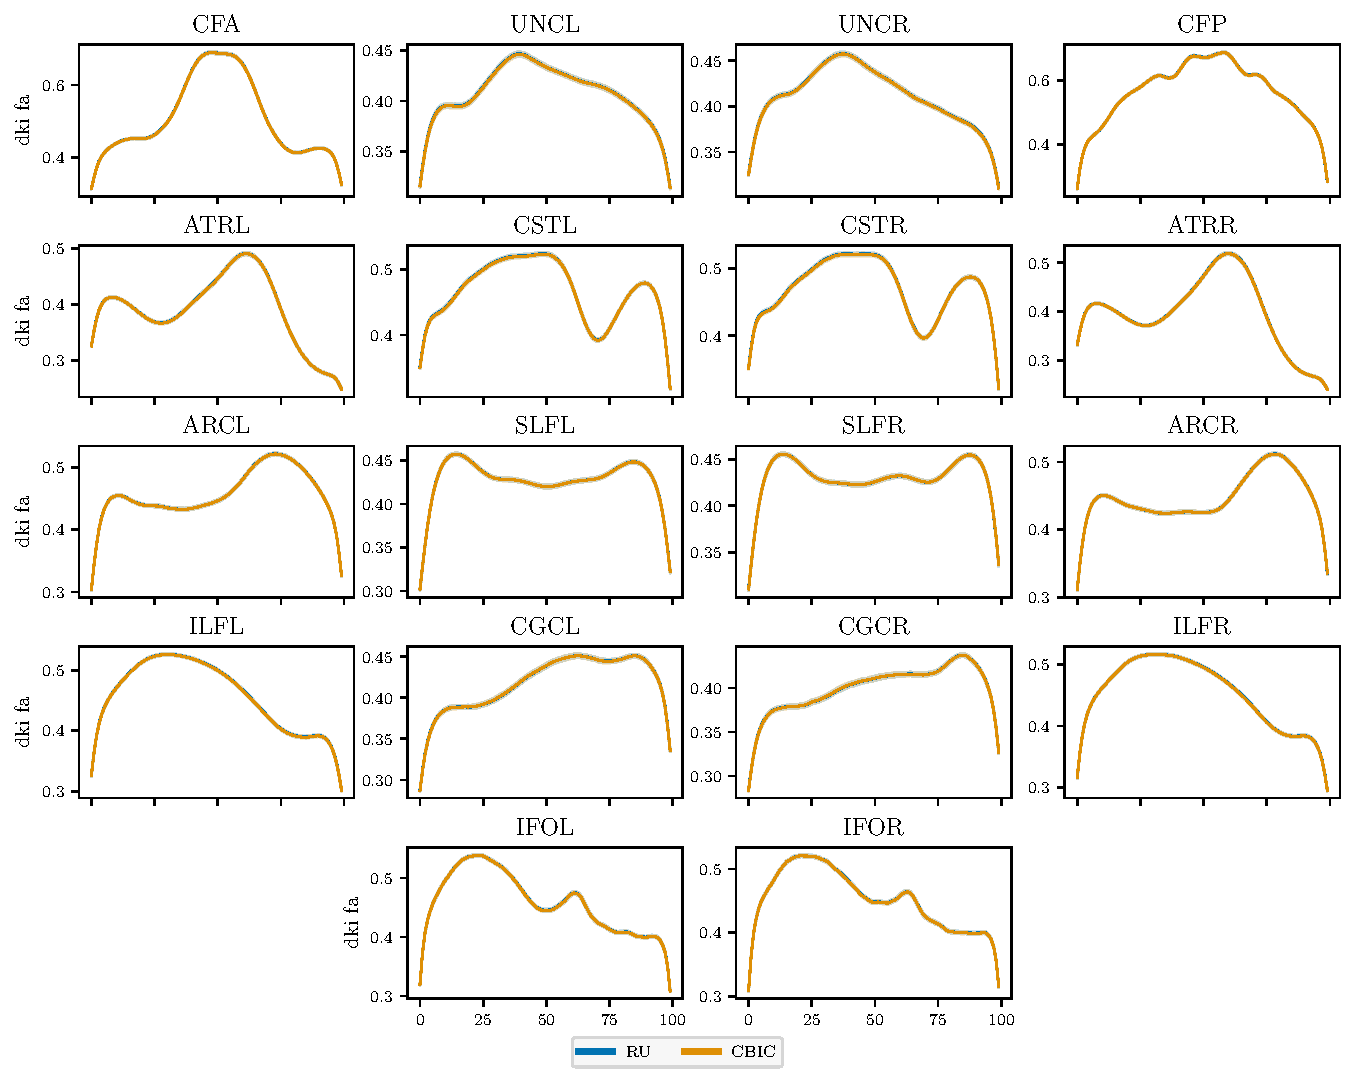
\includegraphics[width=0.9\textwidth]{hbn_harmonized_profiles_fa.pdf}
    \caption{%
        {%
            \bf Site differences in fractional anisotropy (FA)
            do not survive ComBat harmonization.
        }
        \label{fig:hbn-harmonized-bp:fa}
    }
\end{figure}

\begin{figure}
    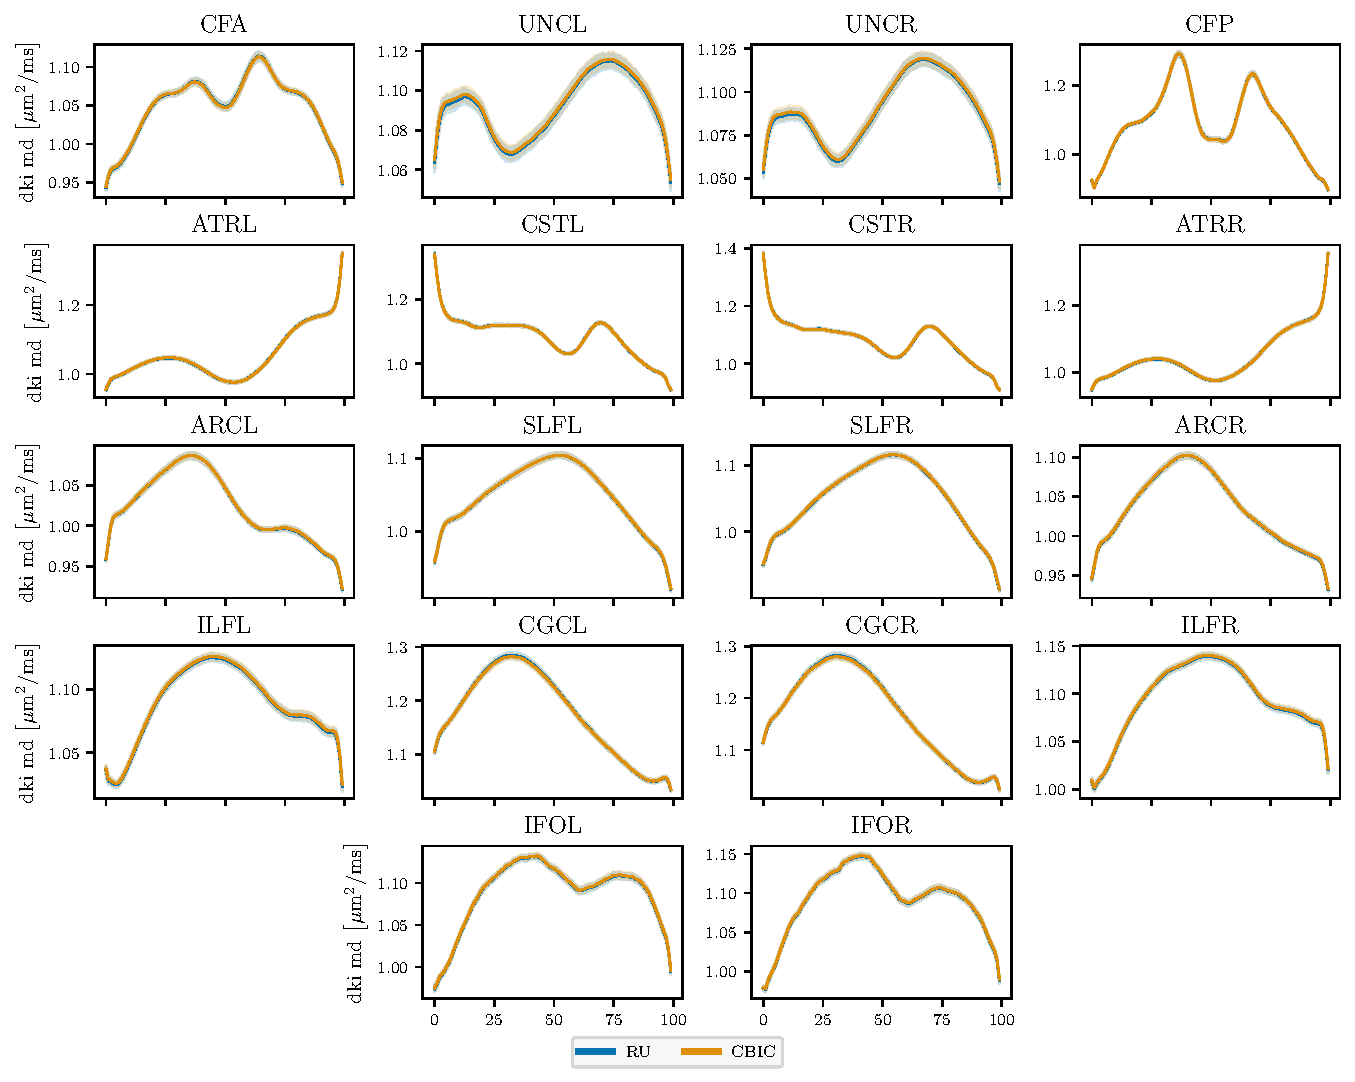
\includegraphics[width=0.9\textwidth]{hbn_harmonized_profiles_md.pdf}
    \caption{%
        {%
            \bf Site differences in mean diffusivity (MD)
            do not survive ComBat harmonization.
        }
        \label{fig:hbn-harmonized-bp:md}
    }
\end{figure}

\pagebreak

\bibliography{paper}

\end{document}
